\section{Diagrammi dei package}
I diagrammi dei package\g~ descrivono le dipendenze che intercorrono tra i vari package\g~ che compongono il sistema.\\
Una dipendenza tra due package\g~ si ha quando una modifica di uno può causare una modifica nell'altro.
Di seguito è riportato il diagramma dei package\g~ dell'applicazione:
	
	\begin{figure}[h!tbp]
		\centering
		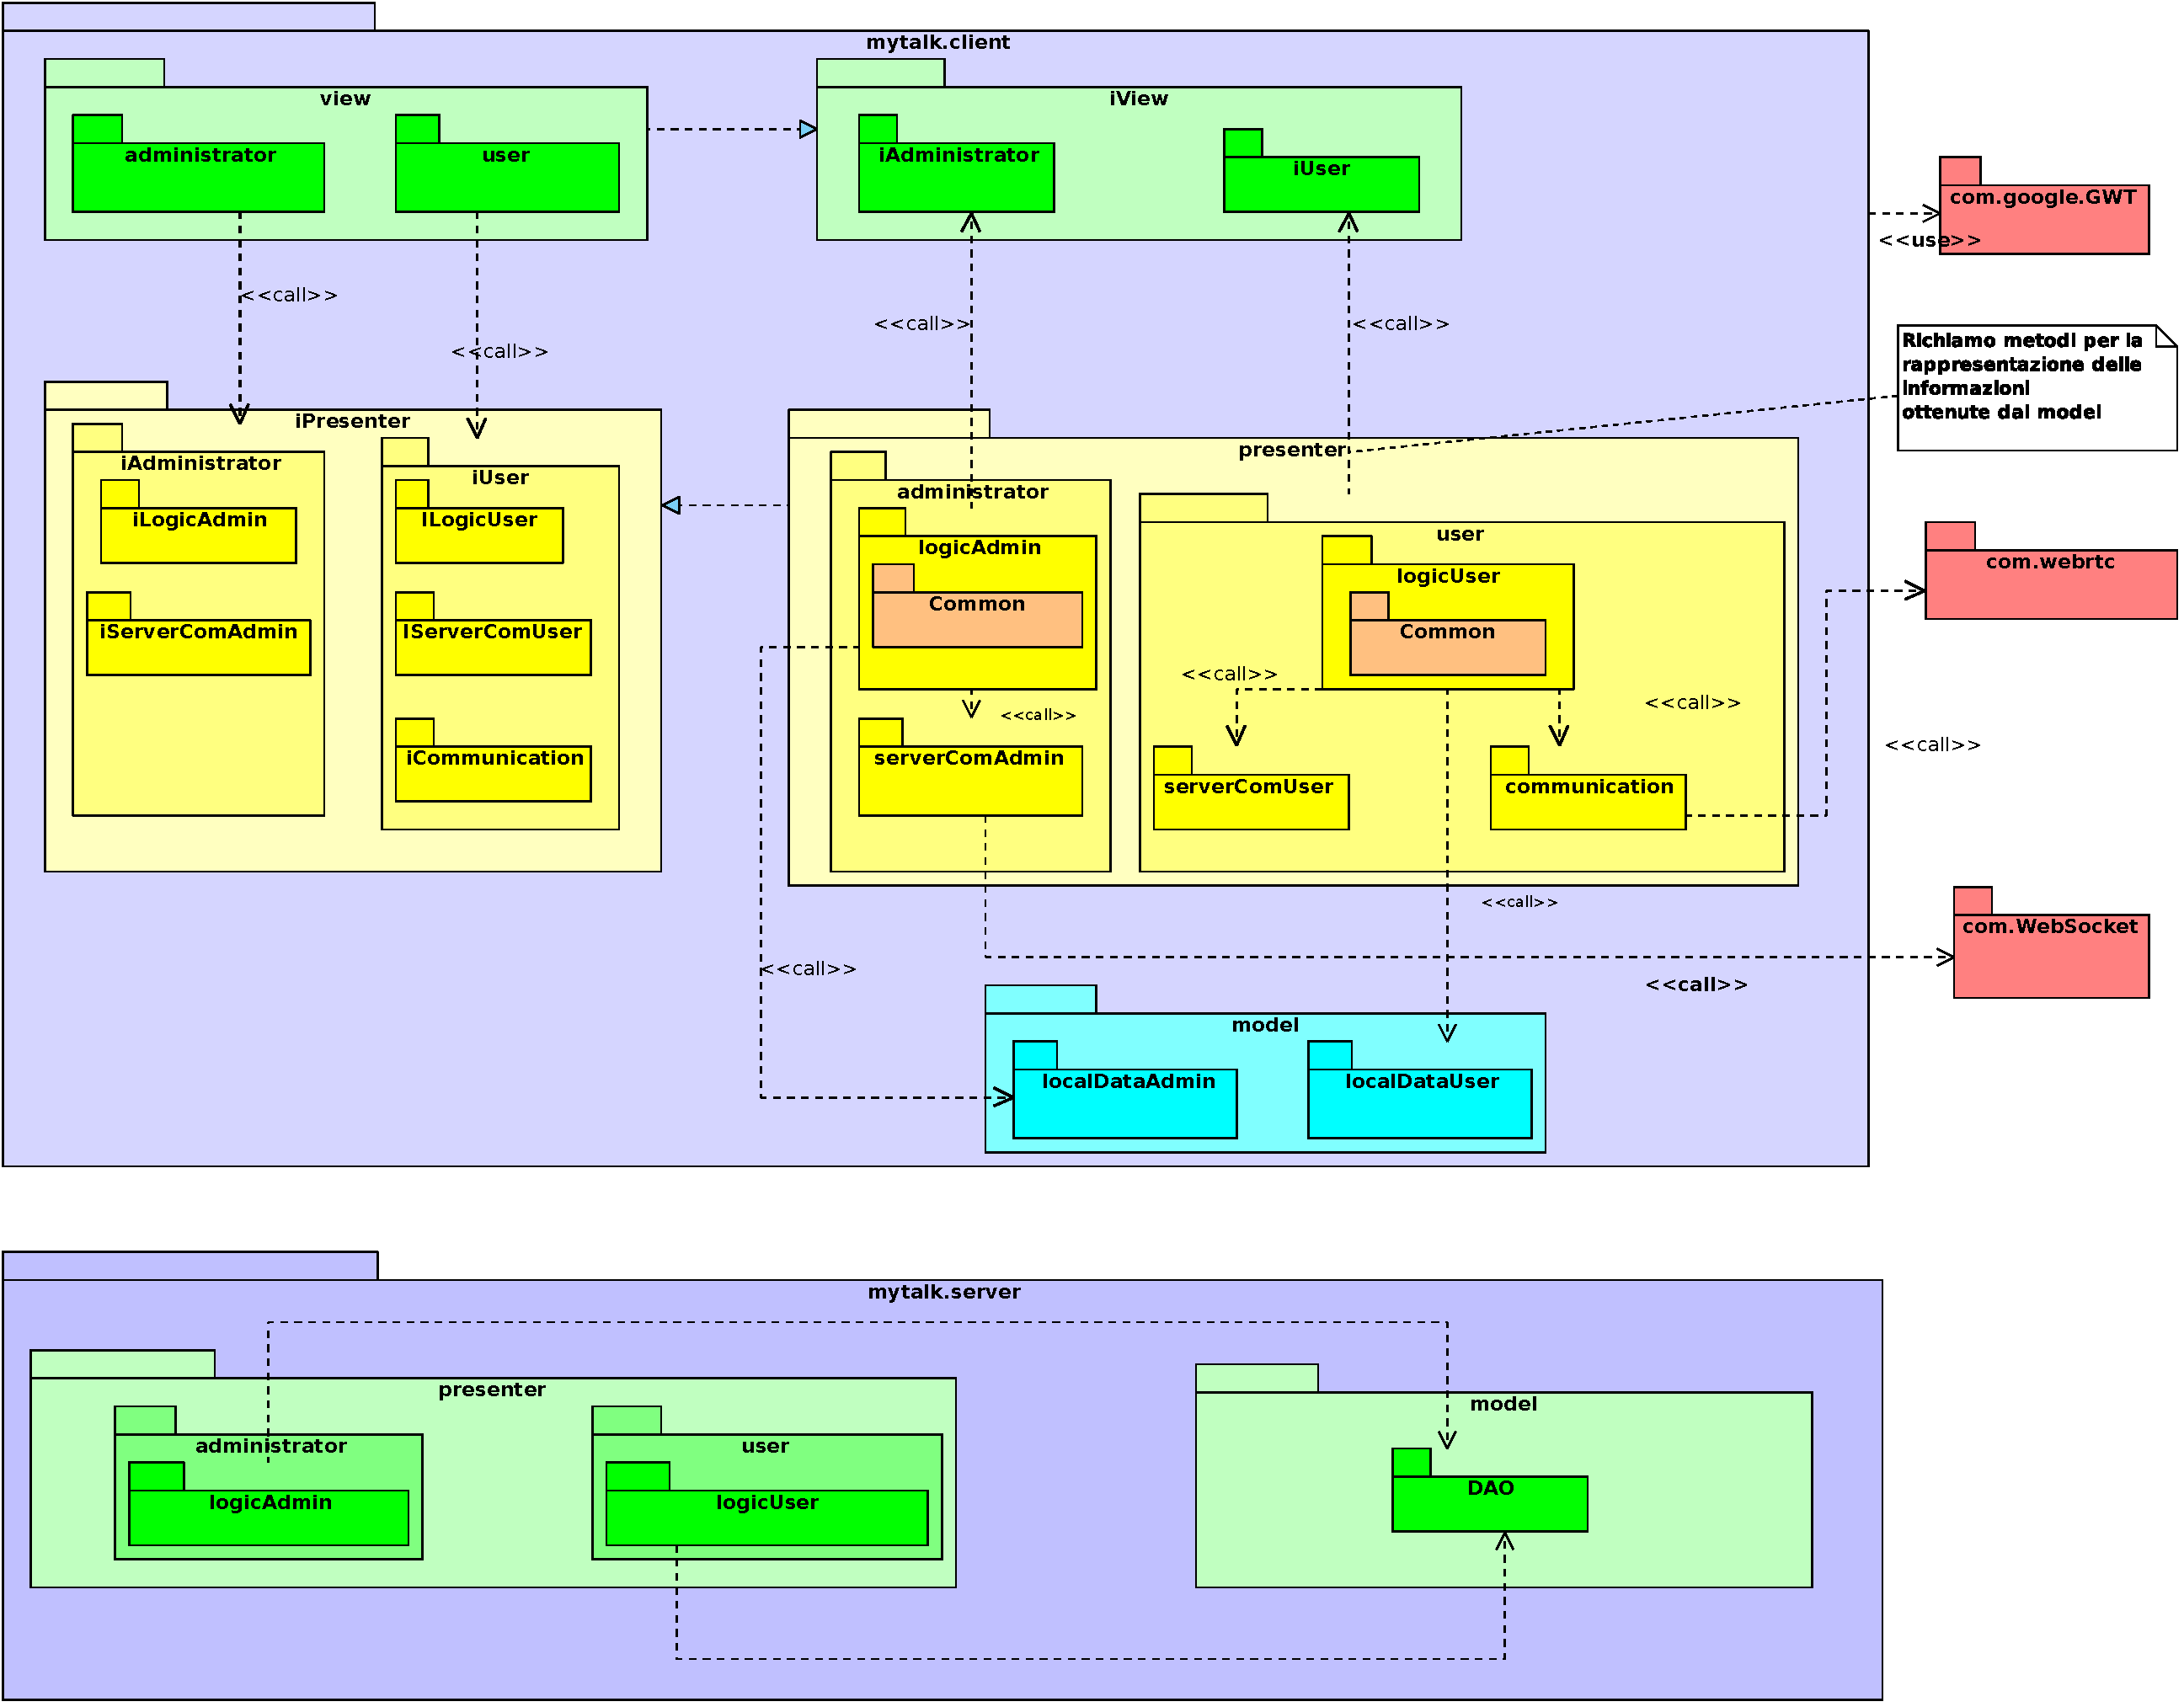
\includegraphics[scale=0.40]{\docsImg dia/MyTalk.pdf}
		\caption{Diagramma dei package del prodotto MyTalk.}
	\end{figure}

L'applicazione è costituita da due package\g~ principali;
\begin{enumerate}
	\item \texttt{mytalk.client}: le classi che compongono questo package\g~ costituiscono la componente front-end\g~ dell'applicazione.
	\item \texttt{mytalk.server}: le classi che compongono questo package\g~ costituiscono la componente back-end\g~ dell'applicazione.
\end{enumerate}
La struttura dei sotto-package\g~ del package\g~ \texttt{mytalk.client} ricalca quella del design pattern MVP.\\
I sotto-package\g~ che compongono il package\g~ \texttt{mytalk.client} sono:
\begin{itemize}
	\item \texttt{mytalk.client.view}: è la componente View del design pattern MVP, implementa il package \texttt{mytalk.client.iView};
	\item \texttt{mytalk.client.presenter}: è la componente Presenter del design pattern MVP, implementa il package \texttt{mytalk.client.iPresenter};
	\item \texttt{mytalk.client.model}: ricalca la componente Model del design pattern MVP;
	\item \texttt{mytalk.client.iView}: contiene le interfacce implementate poi dalle classi che costituiscono la componente View del design pattern MVP, è implementato da \texttt{mytalk.client.view};
	\item \texttt{mytalk.client.iPresenter}: contiene le interfacce implementate poi dalle classi che costituiscono la componente Presenter del design pattern MVP, è implementato da \texttt{mytalk.client.presenter}.
\end{itemize}
I sotto-package\g~ che compongono il package\g~ \texttt{mytalk.server} sono:
\begin{itemize}
	\item \texttt{mytalk.server.presenter};
	\item \texttt{mytalk.server.model}.
\end{itemize}


\subsection{Package mytalk.client.view}
Il package\g~ \texttt{mytalk.client.view} contiene i seguenti sotto-package\g :
\begin{itemize}
	\item \texttt{mytalk.client.view.administrator}: contiene gli elementi necessari a gestire l'interfaccia grafica e a generare gli eventi della parte grafica dell'amministratore.
	\item \texttt{mytalk.client.view.user}: contiene gli elementi necessari a gestire l'interfaccia grafica e a generare gli eventi della parte grafica dell'utente.
\end{itemize} 

\subsection{Package mytalk.client.iView}
Il package\g~ \texttt{mytalk.client.iView} contiene i seguenti sotto-package\g :
\begin{itemize}
	\item \texttt{mytalk.client.iView.iAdministrator}: contiene le interfacce che verranno poi implementate dalle classi che gestiranno l'interfaccia grafica dell'amministratore;
	\item \texttt{mytalk.client.iView.iUser}: contiene le interfacce che verranno poi implementate dalle classi che gestiranno l'interfaccia grafica dell'utente.
\end{itemize} 

\subsection{Package mytalk.client.presenter}
Il package\g~ \texttt{mytalk.client.presenter} contiene tutte le classi del Presenter che risiedono nella parte client\g . Il package \g~ contiene i seguenti sotto-package\g:

%----------------------------------------------------------------------------------------------------------
%MYTALK.CLIENT.PRESENTER
%----------------------------------------------------------------------------------------------------------
\begin{itemize}
	\item \texttt{mytalk.client.presenter.administrator}: \\contiene tutti i package\g~ e le classi che costituiscono la componente Presenter per l'amministratore, il package\g~ è diviso nei seguenti sotto-package\g:
		\begin{itemize}
			\item \texttt{mytalk.client.presenter.administrator.logicAdmin}: \\gestisce gli eventi che sono generati dal package\g~ \\ \texttt{mytalk.client.view.administrator} e aggiorna la componente grafica dell'amministratore;
			\item \texttt{mytalk.client.presenter.administrator.serverComAdmin}:\\contiene le componenti che servono ad interfacciarsi al server\g .
			\item \texttt{mytalk.client.presenter.administrator.common}:\\ contiene le componenti in comune tra i vari package\g~ che compongono la componente presenter.administrator.
		\end{itemize} 
	\item \texttt{mytalk.client.presenter.user}: \\contiene tutti i package\g e le classi che costituiscono la componente Presenter per l'amministratore, il package\g~ è diviso nei seguenti sotto-package\g:
		\begin{itemize}
			\item \texttt{mytalk.client.presenter.user.logicUser}:\\ gestisce gli eventi che sono generati dal package\g~ \texttt{mytalk.view.user} e aggiorna la componente grafica dell'utente;
			\item \texttt{mytalk.client.presenter.user.serverComUser}:\\contiene le componenti che servono ad interfacciarsi al server\g ;
			\item \texttt{mytalk.client.presenter.user.communication}:\\contiene le componenti che servono ad instaurare, gestire ed eventualmente chiudere la chiamata\g ;
			\item \texttt{mytalk.client.presenter.user.logicUser.common}:\\ contiene le componenti in comune tra i vari package\g~ che compongono la componente presenter.user.
		\end{itemize} 
	\end{itemize}
	Della componente Presenter fanno parte anche le librerie WebRTC\g~ individuate dal package\g~ \texttt{com.google.WebRTC} e le librerie WebSocket\g~ individuate dal package\g~ \texttt{com.WebSocket}.
	
	
	
\subsection{Package mytalk.client.iPresenter}
Il package\g~ \texttt{mytalk.client.iPresenter} contiene tutte le interfacce del Presenter che risiedono nella parte client\g . Il package \g~ contiene i seguenti sotto-package\g:

%----------------------------------------------------------------------------------------------------------
%MYTALK.CLIENT.PRESENTER
%----------------------------------------------------------------------------------------------------------
\begin{itemize}
	\item \texttt{mytalk.client.iPresenter.iAdministrator}: \\contiene tutte le interfacce che costituiscono la componente Presenter per l'amministratore, il package\g~ è diviso nei seguenti sotto-package\g:
		\begin{itemize}
			\item \texttt{mytalk.client.iPresenter.iAdministrator.iLogicAdmin}: \\fornisce le interfacce che verranno poi implementate dalle classi contenute nel package\g \\ \texttt{mytalk.client.presenter.administrator.logicAdmin};
			\item \texttt{mytalk.client.iPresenter.iAdministrator.iServerComAdmin}: \\fornisce le interfacce che verranno poi implementate dalle classi contenute nel package\g \\ \texttt{mytalk.client.presenter.administrator.serverComAdmin}.
		\end{itemize} 
	\item \texttt{mytalk.client.iPresenter.iUser}: \\contiene tutte le interfacce che costituiscono la componente Presenter per l'amministratore, il package\g~ è diviso nei seguenti sotto-package\g:
		\begin{itemize}
			\item \texttt{mytalk.client.iPresenter.iUser.iLogicUser}:\\ fornisce le interfacce che saranno poi implementate dal package\g~ \\ \texttt{mytalk.client.presenter.user.logicUser};
			\item \texttt{mytalk.client.presenter.iUser.iServerComUser}:\\ fornisce le interfacce che saranno poi implementate dal package\g~ \\ \texttt{mytalk.client.presenter.user.serverComUser};
			\item \texttt{mytalk.client.presenter.iUser.iCommunication}:\\ fornisce le interfacce che saranno poi implementate dal package\g~ \\ \texttt{mytalk.client.presenter.iUser.iCommunication};
		\end{itemize} 
	\end{itemize}	
	
	
	
\subsection{Package mytalk.client.model}	
Il package\g~ \texttt{mytalk.client.model} contiene tutte le classi del Model che risiedono nella parte client\g . Il package\g~ contiene i seguenti sotto-package\g:
	\begin{itemize}
		\item \texttt{mytalk.client.model.localDataAdmin}: \\contiene le informazioni relative ad un eventuale amministratore autenticato al servizio;
		\item \texttt{mytalk.client.model.localDataUser}: \\contiene le informazioni relative ad un eventuale utente autenticato al servizio.
	\end{itemize}
	
	
\subsection{Package mytalk.server.presenter}
Il package\g~ contiene tutte le classi del Presenter che risiedono nella parte server\g . Il package\g~ contiene i seguenti sotto-package\g:
	\begin{itemize}
		\item \texttt{mytalk.server.presenter.administrator.logicAdmin}: \\questo package\g~ contiene tutte le classi dell'amministratore che costituiscono la parte Presenter del server\g~;
		\item \texttt{mytalk.server.presenter.user.logicUser}:\\questo package\g~ contiene tutte le classi dell'utente che costituiscono la parte Presenter del server\g~;
	\end{itemize}



\subsection{Package mytalk.server.model}
Il package\g~ \texttt{mytalk.server.model} contiene i seguenti sotto-package\g :
\begin{itemize}
\item \texttt{mytalk.server.model.dao}: questo package\g contiene gli oggetti e le interfacce che servono a gestire il database\g.
\end{itemize}





















